% -*-latex-*-

\title{Orbiter Technical Notes: Planetary axis precession}
\author{Martin Schweiger}
\date{July 19, 2010}

\documentclass[a4paper]{article}
\usepackage[dvips]{graphicx}
\usepackage{amsmath}
\usepackage{amsfonts}
\usepackage{amssymb}
\usepackage{times}
\usepackage{cite}
\usepackage{wasysym}

\newcommand{\ACC}{\ensuremath\mathrm{A}}
\newcommand{\AACC}{\ensuremath\mathrm{T}}
\newcommand{\Euler}{\ensuremath\mathrm{E}}
\renewcommand{\vec}[1]{\ensuremath \mathbf{#1}}
\newcommand{\mat}[1]{\ensuremath \mathsf{#1}}

\begin{document}
\bibliographystyle{unsrt}

%\renewcommand{\vec}[1]{\ensuremath{\mathbf{#1}}}

\newcommand{\vR}[1]{\ensuremath{\vec{R}_{#1}}}
\newcommand{\nR}[1]{\ensuremath{|\vR{#1}|}}

\maketitle

\section{Introduction}
This document describes the implementation of planetary axis precession in Orbiter.

\section{Definitions}
The rotation axis of a celestial body is assumed to rotate around a \emph{precession reference axis} at constant obliquity angle and constant angular velocity. Currently, the orientation of the reference axis (OP) is considered time-invariant and is defined with respect to the ecliptic and equinox of J2000 (see Fig.~\ref{fig:prec_ref}). The axis orientation is defined by the obliquity $\varepsilon_\mathrm{ref}$ (the angle between the axis and the ecliptic north pole, $N$) and the angle from the vernal equinox  $\vernal$ to the ascending node of the ecliptic with respect to the body equator, $L_\mathrm{ref}$.
In Orbiter's left-handed system, $\vernal$ is defined as (1,0,0), and $N$ is defined as (0,1,0). The rotation matrix $\mat{R}_\mathrm{ref}$ for transforming from ecliptic to precession reference frame is then given by
\begin{equation}
\mat{R}_\mathrm{ref} = \left( \begin{array}{ccc}
\cos L_\mathrm{ref} & 0 & -\sin L_\mathrm{ref} \\
0 & 1 & 0 \\
\sin L_\mathrm{ref} & 0 & \cos L_\mathrm{ref} \end{array} \right)
\left( \begin{array}{ccc}
1 & 0 & 0 \\
0 & \cos\varepsilon_\mathrm{ref} & -\sin\varepsilon_\mathrm{ref} \\
0  & \sin\varepsilon_\mathrm{ref} & \cos\varepsilon_\mathrm{ref}
\end{array} \right).
\end{equation}
\begin{figure}[ht]
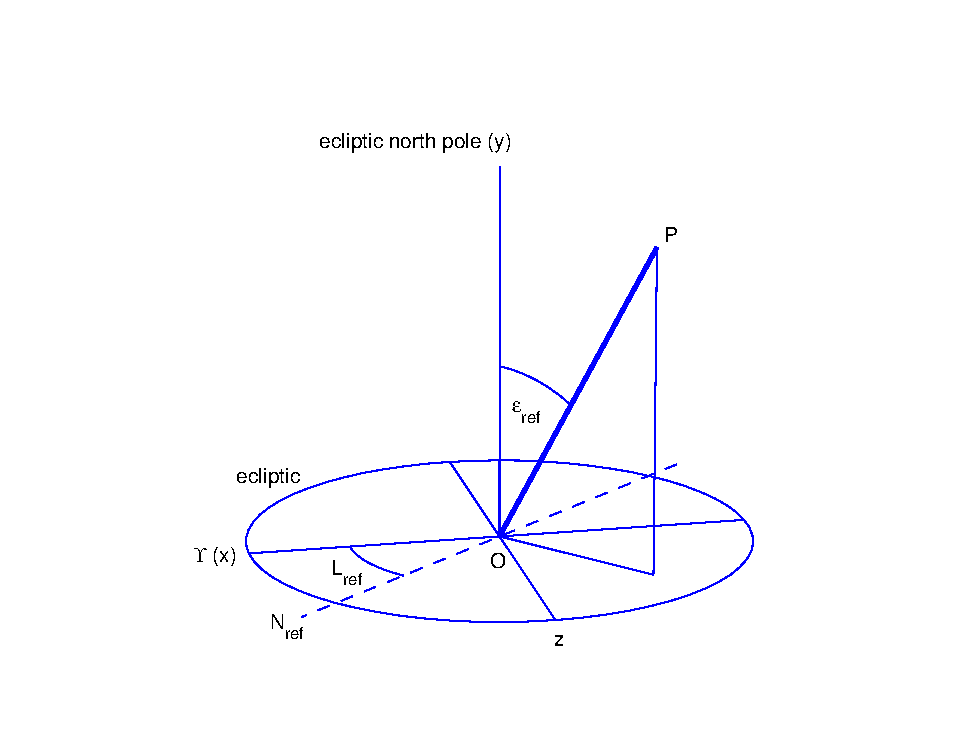
\includegraphics[width=\textwidth]{fig1.eps}
\caption{Orientation of the precession reference axis in the ecliptic frame.}
\label{fig:prec_ref}
\end{figure}
The planet's axis of rotation at some time $t$, OS, is given relative to the reference axis OP, by obliquity $\varepsilon_\mathrm{rel}$ and longitude $L_\mathrm{rel}$ (see Fig.~\ref{fig:prec_ecl}). $L_\mathrm{rel}$ is a linear function of time, and is defined as
\begin{equation}
L_\mathrm{rel}(t) = L_0 + 2\pi \frac{t-t_0}{T_p},
\end{equation}
where $t_0$ is a reference date, $L_0$ is the longitude at that date, and $T_p$ is the precession period.
The rotation from the precession reference frame to the planet's axis frame is described by
\begin{equation}
\mat{R}_\mathrm{rel}(t) = \left(\begin{array}{ccc}
\cos L_\mathrm{rel} & 0 & -\sin L_\mathrm{rel} \\
0 & 1 & 0 \\
\sin L_\mathrm{rel} & 0 & \cos L_\mathrm{rel}
\end{array} \right)
\left(\begin{array}{ccc}
1 & 0 & 0 \\
0 & \cos \varepsilon_\mathrm{rel} & -\sin \varepsilon_\mathrm{rel} \\
0 & \sin \varepsilon_\mathrm{rel} & \cos \varepsilon_\mathrm{rel}
\end{array} \right).
\end{equation}
\begin{figure}[ht]
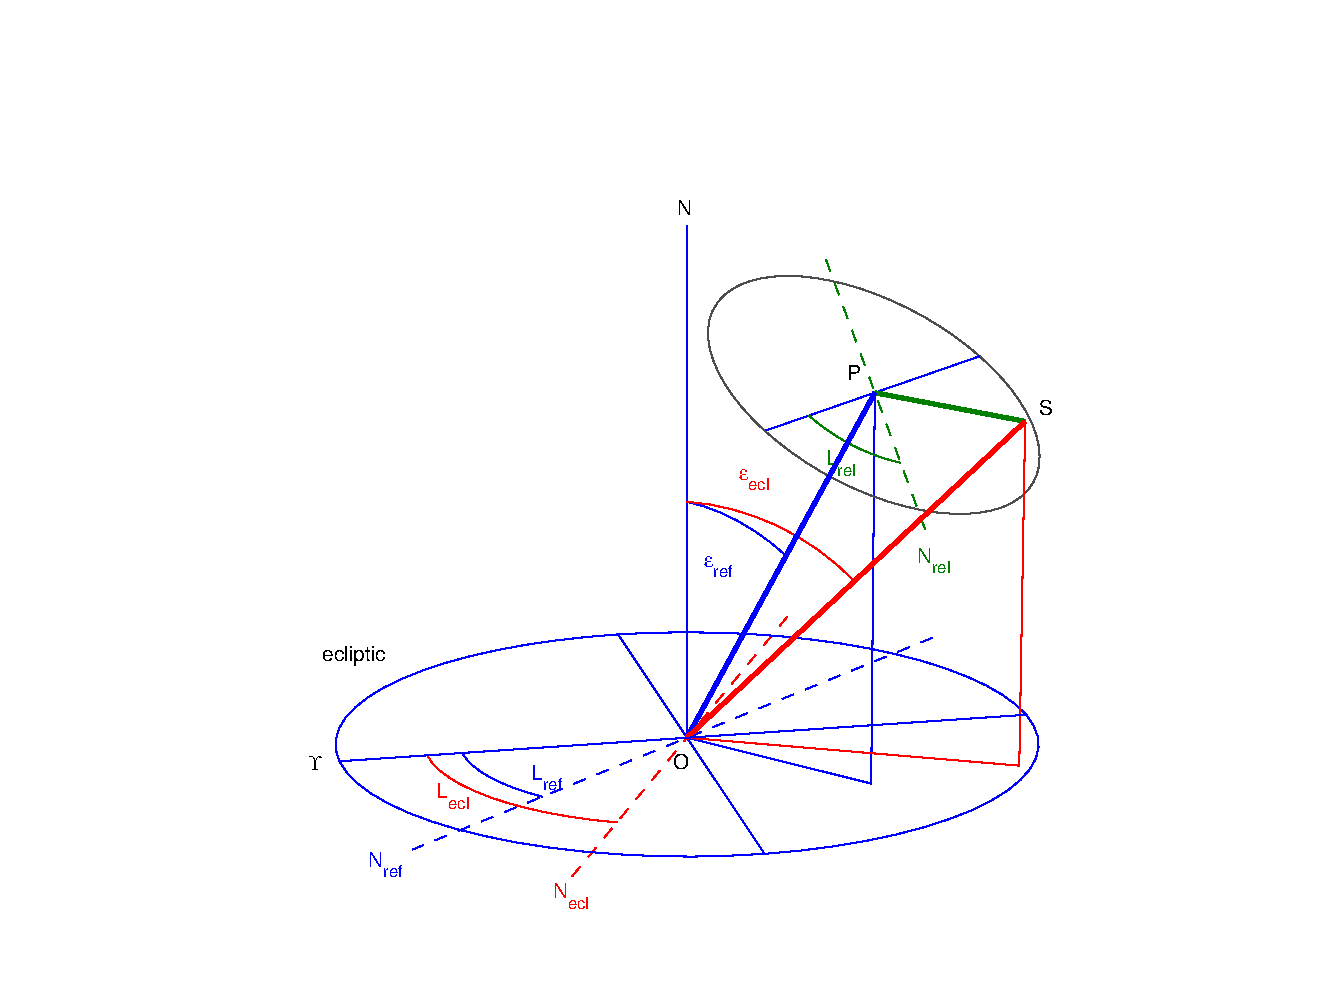
\includegraphics[width=\textwidth]{fig2.eps}
\caption{Planet rotation axis.}
\label{fig:prec_ecl}
\end{figure}
The planet's rotation angle $\varphi(t)$ is defined via the siderial period $T_s$, and a rotation offset $\varphi_0$:
\begin{equation}\label{eq:rotation}
\varphi(t) = \varphi_0 + 2\pi \frac{t-t_0}{T_s} + [L_0 - L_\mathrm{rel}(t)] \cos \varepsilon_\mathrm{rel},
\end{equation}
where $t_0$ is a reference time (usually J2000.0). The last term in Eq.~\ref{eq:rotation} accounts for the difference between siderial and node-to-node rotation period.
The rotation is encoded in matrix $\mat{R}_\mathrm{rot}$:
\begin{equation}
\mat{R}_\mathrm{rot}(t) = \left( \begin{array}{ccc}
\cos\varphi & 0 & -\sin\varphi \\
0 & 1 & 0 \\
\sin\varphi & 0 & \cos\varphi
\end{array} \right).
\end{equation}
The full planet transformation is the combination of rotation and precession:
\begin{equation}\label{eq:fullrot}
\mat{R}(t) = \mat{R}_\mathrm{ref} \mat{R}_\mathrm{rel}(t) \mat{R}_\mathrm{rot}(t).
\end{equation}
The direction of the rotation axis is
\begin{equation}
\mathrm{OS}: \vec{s}(t) = \mat{R}(t) \left(\begin{array}{c}
0 \\ 1 \\ 0 \end{array}\right).
\end{equation}
The resulting axis obliquity and longitude of ascending node are
\begin{equation}\label{eq:eps_ecl}
\varepsilon_\mathrm{ecl}(t) = \cos^{-1} s_y(t), \qquad
L_\mathrm{ecl}(t) = \tan^{-1} \frac{-s_x(t)}{s_z(t)}.
\end{equation}
Figure \ref{fig:plots} shows examples of axis obliquity and longitude of ascending node over one precession cycle for different reference obliquities, as a function of $L_\mathrm{rel}$ (or equivalently, time).
\begin{figure}
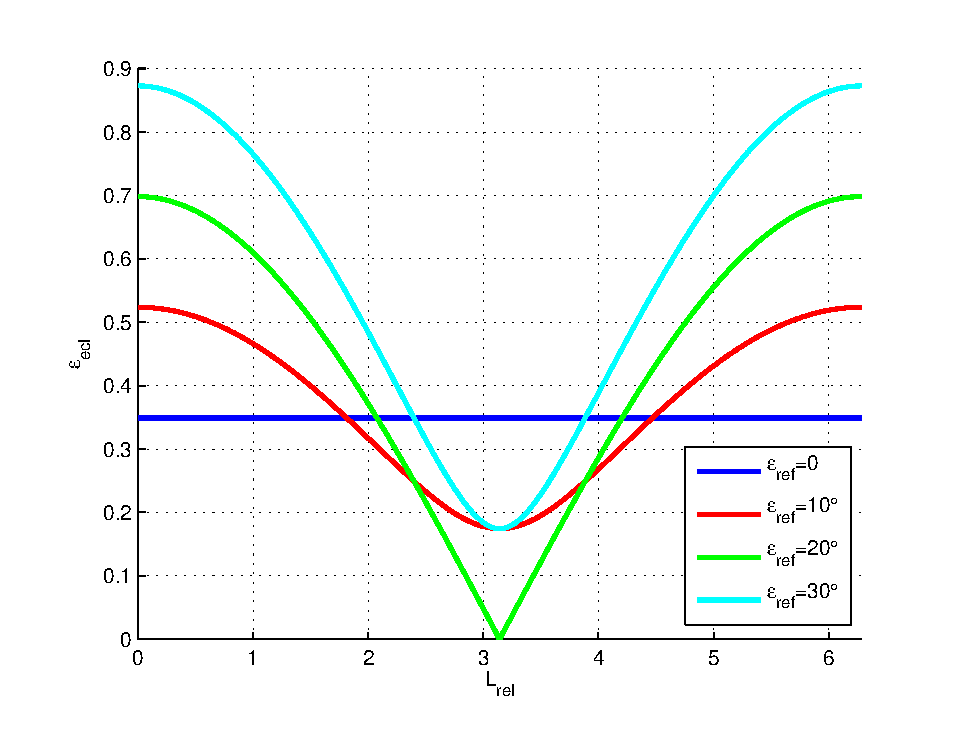
\includegraphics[width=0.5\textwidth]{fig3a.eps}
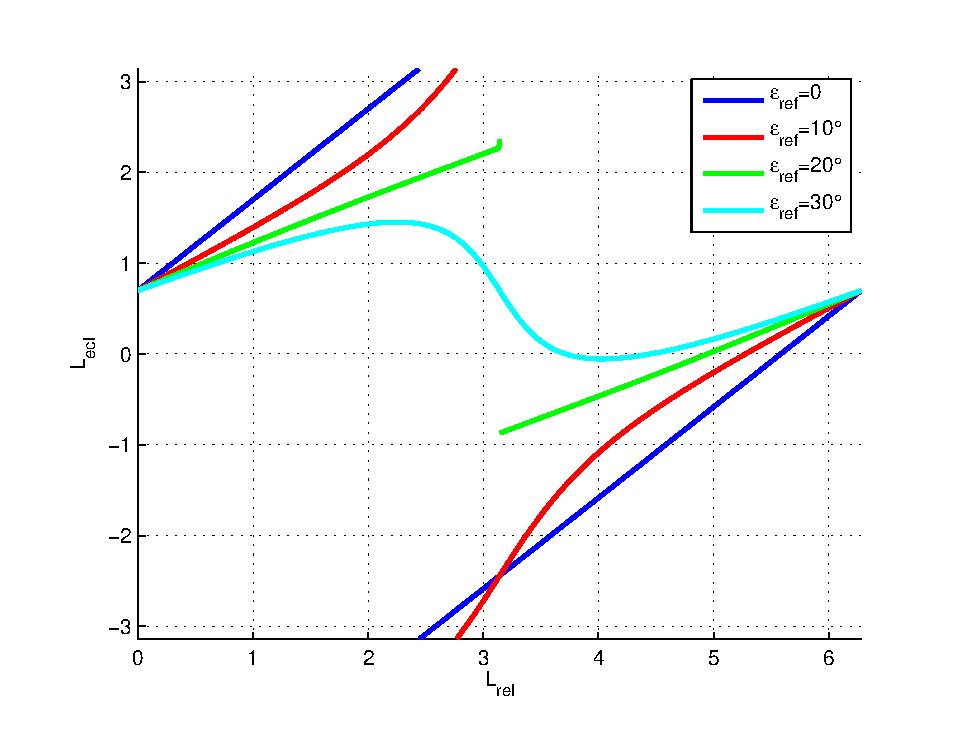
\includegraphics[width=0.5\textwidth]{fig3b.eps}
\caption{Axis obliquity $\varepsilon_\mathrm{ecl}$ and longitude of ascending node $L_\mathrm{ecl}$ as a function of relative longitude $L_\mathrm{rel}$ over one precession cycle, for four different values of $\varepsilon_\mathrm{ref}$, and invariant parameters $\varepsilon_\mathrm{rel} = 20^\circ$, $L_\mathrm{ref}=40^\circ$.}
\label{fig:plots}
\end{figure}
Using $\varepsilon_\mathrm{ecl}$ and $L_\mathrm{ecl}$, an \emph{obliquity matrix} $\mat{R}_\mathrm{ecl}$ can be defined that rotates from ecliptic to the planet's current precession frame:
\begin{equation}\label{eq:rot_ecl}
\mat{R}_\mathrm{ecl}(t) = \left( \begin{array}{ccc}
\cos L_\mathrm{ecl} & 0 & -\sin L_\mathrm{ecl} \\
0 & 1 & 0 \\
\sin L_\mathrm{ecl} & 0 & \cos L_\mathrm{ecl} \end{array} \right)
\left( \begin{array}{ccc}
1 & 0 & 0 \\
0 & \cos\varepsilon_\mathrm{ecl} & -\sin\varepsilon_\mathrm{ecl} \\
0  & \sin\varepsilon_\mathrm{ecl} & \cos\varepsilon_\mathrm{ecl}
\end{array} \right).
\end{equation}
Note that like $\mat{R}_\mathrm{ref} \mat{R}_\mathrm{rel}$, matrix $\mat{R}_\mathrm{ecl}$ describes a rotation of the axis from ON to OS. However, there is a difference between the rotation around OS. Specifically, the reference axis for $\mat{R}_\mathrm{ecl}$ is the ascending node of the ecliptic with respect to the planet equator:
\begin{equation}
\mathrm{ON}_\mathrm{ecl}: \vec{n}(t) = \mat{R}_\mathrm{ecl}(t)
\left( \begin{array}{c} 1 \\ 0 \\ 0 \end{array} \right).
\end{equation}
The difference between $\mat{R}_\mathrm{ecl}$ and $\mat{R}_\mathrm{ref} \mat{R}_\mathrm{rel}$ can be expressed by an offset matrix $\mat{R}_\mathrm{off}$:
\begin{eqnarray}
\mat{R}_\mathrm{ecl}(t) \mat{R}_\mathrm{off}(t) &=& \mat{R}_\mathrm{ref} \mat{R}_\mathrm{rel}(t),\\
\mat{R}_\mathrm{off}(t) &=& \mat{R}^T_\mathrm{ecl}(t) \mat{R}_\mathrm{ref} \mat{R}_\mathrm{rel}(t).
\end{eqnarray}
$\mat{R}_\mathrm{off}$ describes a rotation around y, so it has the structure
\begin{equation}
\mat{R}_\mathrm{off}(t) = \left( \begin{array}{ccc}
\cos \varphi_\mathrm{off} & 0 & -\sin \varphi_\mathrm{off} \\
0 & 1 & 0 \\
\sin \varphi_\mathrm{off} & 0 & \cos \varphi_\mathrm{off} \end{array} \right),
\end{equation}
and the offset angle $\varphi_\mathrm{off}$ is given by
\begin{equation}
\varphi_\mathrm{off}(t) = \tan^{-1} \frac{-[\mat{R}_\mathrm{off}]_{13}}{[\mat{R}_\mathrm{off}]_{11}}.
\end{equation}
Including this offset into the planet's rotation angle leads to an expression for the planet's rotation angle $r(t)$ with respect to reference direction $\vec{n}(t)$:
\begin{equation}\label{eq:rotangle}
r(t) = \varphi(t) + \varphi_\mathrm{off}(t).
\end{equation}
We can now express the full rotation matrix $\mat{R}$ defined in Eq.~\ref{eq:fullrot}, using $\mat{R}_\mathrm{ecl}$ and $r$:
\begin{equation}
\mat{R}(t) = \mat{R}_\mathrm{ecl}(t) \tilde{\mat{R}}_\mathrm{rot}(t),
\end{equation}
where
\begin{equation}
\tilde{\mat{R}}_\mathrm{rot}(t) = \left( \begin{array}{ccc}
\cos r & 0 & -\sin r \\
0 & 1 & 0 \\
\sin r & 0 & \cos r
\end{array} \right).
\end{equation}

\section{Orbiter interface}
\subsection{Configuration}
The precession and rotation parameters supported in planet configuration files are listed in Table~\ref{tab:param}.
The following default assumptions apply:
\begin{itemize}
\item If PrecessionObliquity is not specified, $\varepsilon_\mathrm{ref}=0$ is assumed. (precession reference is ecliptic normal). In this case, the $L_\mathrm{ref}$ entry is ignored and $L_\mathrm{ref}=0$ is assumed.
\item If PrecessionPeriod is not specified, $T_p = \infty$ is assumed (rotation axis is stationary).
\item If LAN\_MJD is not specified, $t_0 = 51544.5$ is assumed (J2000.0).
\item If LAN is not specified, $L_0=0$ is assumed.
\item If Obliquity is not specified, $\varepsilon_\mathrm{rel}=0$ is assumed.
\item If SidRotPeriod is not specified, $T_s=\infty$ is assumed (no rotation).
\item If SidRotOffset is not specified, $\varphi_0=0$ is assumed.
\end{itemize}
For a retrograde precession of the equinoxes, a negative value of PrecessionPeriod should be used.

\begin{table}[hb]
\begin{tabular}{ll}
parameter & config entry \\ \hline
$T_s$ & SidRotPeriod [seconds] \\
$\varphi_0$ & SidRotOffset [rad] \\
$\varepsilon_\mathrm{rel}$ & Obliquity [rad] \\
$L_0$ & LAN [rad] \\
$t_0$ & LAN\_MJD [MJD] \\
$T_p$ & PrecessionPeriod [days] \\
$\varepsilon_\mathrm{ref}$ & PrecessionObliquity [rad] \\
$L_\mathrm{ref}$ & PrecessionLAN [rad]
\end{tabular}
\caption{Rotation and precession parameter entries in planet configuration files.}
\label{tab:param}
\end{table}

\subsection{API functions}
\subsubsection{void oapiGetPlanetObliquityMatrix (OBJHANDLE hPlanet, MATRIX3 *mat)}
This function returns $\mat{R}_\mathrm{ecl}(t)$ in Eq.~\ref{eq:rot_ecl} for planet \emph{hPlanet} at the current simulation time.

\subsubsection{double oapiGetPlanetObliquity (OBJHANDLE hPlanet)}
This function returns $\varepsilon_\mathrm{ecl}(t)$ in Eq.~\ref{eq:eps_ecl} for planet \emph{hPlanet} at the current simulation time.

\subsubsection{double oapiGetPlanetTheta (OBJHANDLE hPlanet)}
This function returns $L_\mathrm{ecl}(t)$ in Eq.~\ref{eq:eps_ecl} for planet \emph{hPlanet} at the current simulation time.

\subsubsection{double oapiGetPlanetCurrentRotation (OBJHANDLE hPlanet)}
This function returns the current rotation angle $r(t)$ in Eq.~\ref{eq:rotangle} for planet \emph{hPlanet} at the current simulation time.

\subsubsection{void oapiGetRotationMatrix (OBJHANDLE hPlanet, MATRIX3 *mat)}
This function returns $\mat{R}(t)$ in Eq.~\ref{eq:fullrot} for planet \emph{hPlanet} at the current simulation time.

\end{document}
